\documentclass[11pt,letterpaper]{article}

%% === margins ===
%\addtolength{\hoffset}{-0.75in} \addtolength{\voffset}{-0.75in}
%\addtolength{\textwidth}{1.5in} \addtolength{\textheight}{1.6in}
%% === basic packages ===
\usepackage{latexsym}
\usepackage{amssymb,amsmath}
\usepackage{graphicx}
\usepackage{verbatim}
\usepackage{ccaption}
\usepackage{booktabs}
%% === bibliography packages ===
\usepackage{natbib}
\bibliographystyle{asa}
%% === hyperref options ===
\usepackage{color}
\usepackage[table]{xcolor}
\usepackage{graphicx} 
\usepackage{booktabs} 
\usepackage{xcolor}
\usepackage{colortbl}
\usepackage{multirow}
\usepackage{amsmath}
\usepackage{rotating}
\usepackage{lscape}
\usepackage{longtable}
\usepackage{subfig}
\usepackage[pdftex, bookmarksopen=true, bookmarksnumbered=true, 
pdfstartview=FitH, breaklinks=true, urlbordercolor={1 1 1}, citebordercolor={1 1 1}]{hyperref}  
\usepackage{lipsum} %package to eliminate pagenumbering, using \pagenumbering{gobble}
% === dcolumn package ===
\usepackage{dcolumn}
\newcolumntype{.}{D{.}{.}{-1}}
\newcolumntype{d}[1]{D{.}{.}{#1}}
% === theorem package ===
\usepackage{theorem}
\theoremstyle{plain}
\theoremheaderfont{\scshape}
\newtheorem{proposition}{Proposition}
\newtheorem{assumption}{Assumption}
\def\qed{\hfill \vrule height7.5pt width6.17pt depth0pt}

\renewcommand{\arraystretch}{1.2}
\newcolumntype{R}[1]{>{\currentrowstyle\raggedleft\arraybackslash}p{#1}}

% ==== rotating package ===
\usepackage{rotating}

% ==== threeparttable package ===
\usepackage[para]{threeparttable}

% == spacing between sections and subsections
\usepackage[compact]{titlesec} 

\newtheorem{theorem}{Theorem}
%\newtheorem{proposition}[theorem]{Proposition}
\newtheorem{corollary}[theorem]{Corollary}
\newtheorem{lemma}[theorem]{Lemma}
\newtheorem{definition}{Definition}
\theoremstyle{remark}
\newtheorem{rem}{Remark}

\newcommand{\itl}{\textit}
\newcommand{\beg}{\begin}
\newcommand{\tbf}{\textbf}
\newcommand{\non}{\nonumber}
\newcommand{\noi}{\noindent}
\newcommand{\bs}{\bigskip}
\newcommand{\tcr}[1]{\textcolor{red}{#1}}
\newcommand{\tcb}[1]{\textcolor{blue}{#1}}
\newcommand{\hlight}[1]{\colorbox{yellow}{#1}}
\newcommand{\ds}{\displaystyle}
\definecolor{Gray}{gray}{0.9}

\textwidth=16cm \textheight=23cm
%\parskip=\medskipamount
\parindent=0.3in
\topmargin=-2cm \oddsidemargin=0cm

\numberwithin{equation}{section}

\begin{document}

\newcommand\spacingset[1]{\renewcommand{\baselinestretch}%
{#1}\small\normalsize}
\spacingset{1}

\newcommand{\blind}{0} \newcommand{\tit}{Supplementary Materials for ``Quantifying the Contribution of Earlier Detection and Advancements in Treatment on Gains in Life Expectancy for US Breast Cancer Patients Since 1975''}
%%%%%%%%%%%%%%%%%%%%%%%%%%%%%%%%%%%%%%%%%%%%%%%%%%%%%%%%%%%%%%%%%%%%%%%%

\if0\blind

 {\title{\bf \tit}
 
  \author{Samir Soneji\thanks{Norris Cotton Cancer Center and
      Dartmouth Institute for Health Policy \& Clinical Practice,
      Geisel School of Medicine at Dartmouth. Email: \href{mailto:samir.soneji@dartmouth.edu}{samir.soneji@dartmouth.edu}}
  \quad \quad 
  Hiram Beltr\'{a}n-S\'{a}nchez\thanks{Community Health Sciences, University of California, Los Angeles. Email:
    \href{mailto:beltrans@ucla.edu}{beltrans@ucla.edu}}}

\date{ }

\maketitle} \fi

% \begin{abstract}
% {\textbf{Background}.  US breast cancer mortality rates declined by 32\% since 1975, although the precise contributions of earlier detection and advancements in breast cancer treatment remain unknown.  We quantify the contributions of these two factors, as well as advancements in the treatment of other diseases, on gains in life expectancy among breast cancer patients.

% \textbf{Methods}.  We obtained annual incidence-based case fatality rates for 664,000 breast cancer patients aged 40 years and older from the Surveillance, Epidemiology, and End Results registries, 1975 to 2012.  We used life-table methods to calculate the gain in life expectancy and quantify the three constituent components of this gain: [1] earlier detection, [2] advancements in breast cancer treatment, and [3] advancements in the treatment of other diseases.  We additionally quantify which age groups contributed the most to the overall contribution of earlier detection.  We assumed a 10\% overdiagnosis level for tumors $\leq$3cm, and varied the level up to 32\% in a sensitivity analysis.

% \textbf{Results}.  Overall,  life expectancy increased 10.94 years between 1975 and 2002 for a 40-year old newly diagnosed breast cancer patient.  Advancements in breast cancer treatment contributed more to the gain in life expectancy than earlier detection: 6.79 years (62\%) versus 2.92 years (27\%).  Advancements in the treatment of other diseases contributed the remaining 1.25 years to this gain (11\%).  By age group, earlier detection among 40-49 year olds contributed more to the overall contribution of earlier detection (0.56 years) than 50-59 and 60-69 year olds (0.45 and 0.41 years, respectively).  We reached nearly identical substantive conclusions varying the level of overdiagnosis.

% \textbf{Conclusion}.  Life expectancy among breast cancer patients increased over time primarily because of advancements in breast cancer treatment, although the contribution of earlier detection was not trivial.}
% \end{abstract}
\if1\blind \title{\bf \tit} \maketitle \fi

\pdfbookmark[1]{Title Page}{Title Page}

\thispagestyle{empty}
\setcounter{page}{0}



\newpage
\clearpage
%%%%%%%%%%%%%%%%%%%%%%%%%%%%%%%%%%%%%%%%%%%%%%%%%%%%%%%%%%%%%%%%%%%%%%
 \setcounter{table}{0}  % reset counter for equation numbers
 \setcounter{figure}{0}  % reset counter for equation numbers
 \setcounter{page}{1}
 \renewcommand{\figurename}{Supplemental Figure}
 \renewcommand{\tablename}{Supplemental Table}
%\clearpage
%\pagenumbering{gobble}
\appendix

\spacingset{1.5}
\section{Computation of Incidence-Based Case Fatality Rates}
An incidence-based case fatality rate for a specific cohort of newly
diagnosed breast cancer patients equals the ratio of [1] the number of
deaths occurring for this cohort up to 10 years beyond their diagnosis
and [2] the total number of person-years lived by this cohort up to 10
years beyond their diagnosis.  For example, 556 women aged 65-69 years
were diagnosed with $<$1 cm breast cancer in 2001.  Between 2001 and
2011, 22 of these women died of breast cancer and another 107 died of
a competing cause of death.  This entire cohort lived a total of
5099.5 person-years over the 10-year period.  Thus, the
incidence-based case fatality rate from breast cancer equaled
22/5099.5 and the incidence-based case fatality rate from competing
causes of death equaled 107/5099.5.

\section{Adjustment for Overdiagnosis}
Suppose 10\% of the 556 women aged 65-69 years old diagnosed with <1cm
breast cancer in 2001 were overdiagnosed, the observed case fatality
rate from breast cancer (22/11,591) would become 22/[11,591 -
0.10*11,591].  Formally, let $m_{a,t,i}$ represent the observed case fatality
rate for age group $a \in \mathcal{A}$ (e.g., 40-44 years, \dots,
$\geq$100 years), year $t \in \mathcal{T}$ (e.g., 1975, \dots 2002), and
tumor size $s \in \mathcal{S}$ (e.g., $<1$
cm, 1-2 cm, 2-3 cm, 3-5 cm, and 5+ cm).  Let $\alpha_i$ represent the assummed
level of overdiagnosis for tumor size $i$. Then, the case fatality
rate adjusted for overdiagnosis, $m^*_{a,t,i}$ equals, $\frac{1}{1-\alpha_i} \times m_{a,t,i}$.

\section{Schematic Representation of the Methodology}
For simplicity, consider three mutually exclusive and exhaustive
categories of tumor size: 1, 2, and 3 (e.g., $<$1cm, 1-2cm, and
$\geq$2cm).  Suppose the distribution of tumor size at cancer
diagnosis remains constant between times 1 and 2
(Figure~\ref{fig:simple_case}, Panel A), tumor size-specific case
fatality rates from breast cancer decrease between times 1 and 2
(Figure~\ref{fig:simple_case}, Panel B), and tumor size-specific case
fatality rates from competing causes of death remain constant between
times 1 and 2 (Figure~\ref{fig:simple_case}, Panel B).  Tumor
size-specific life expectancy increases between times 1 and 2 because
tumor size-specific case fatality rates from breast cancer decreased
over the time period (Figure~\ref{fig:simple_case}, Panel C).  Overall
life expectancy at each time equals the weighted average of tumor
size-specific life expectancy, where the weights equal the
distribution of tumor sizes at cancer diagnosis at times 1 and 2,
respectively.  Overall life expectancy grew between times 1 and 2, and
this gain was entirely due to decreases in tumor size-specific case
fatality rates from breast cancer (Figure~\ref{fig:simple_case}, Panel
D).  In actuality, all three aforementioned factors change over time
and contribute to the gain in life expectancy.  We quantify the
individual contribution of each of these three constituent components.
We also utilize the same demographic method to further disaggregate
these three contributions by age group.
\begin{figure}[!h]
\begin{center}
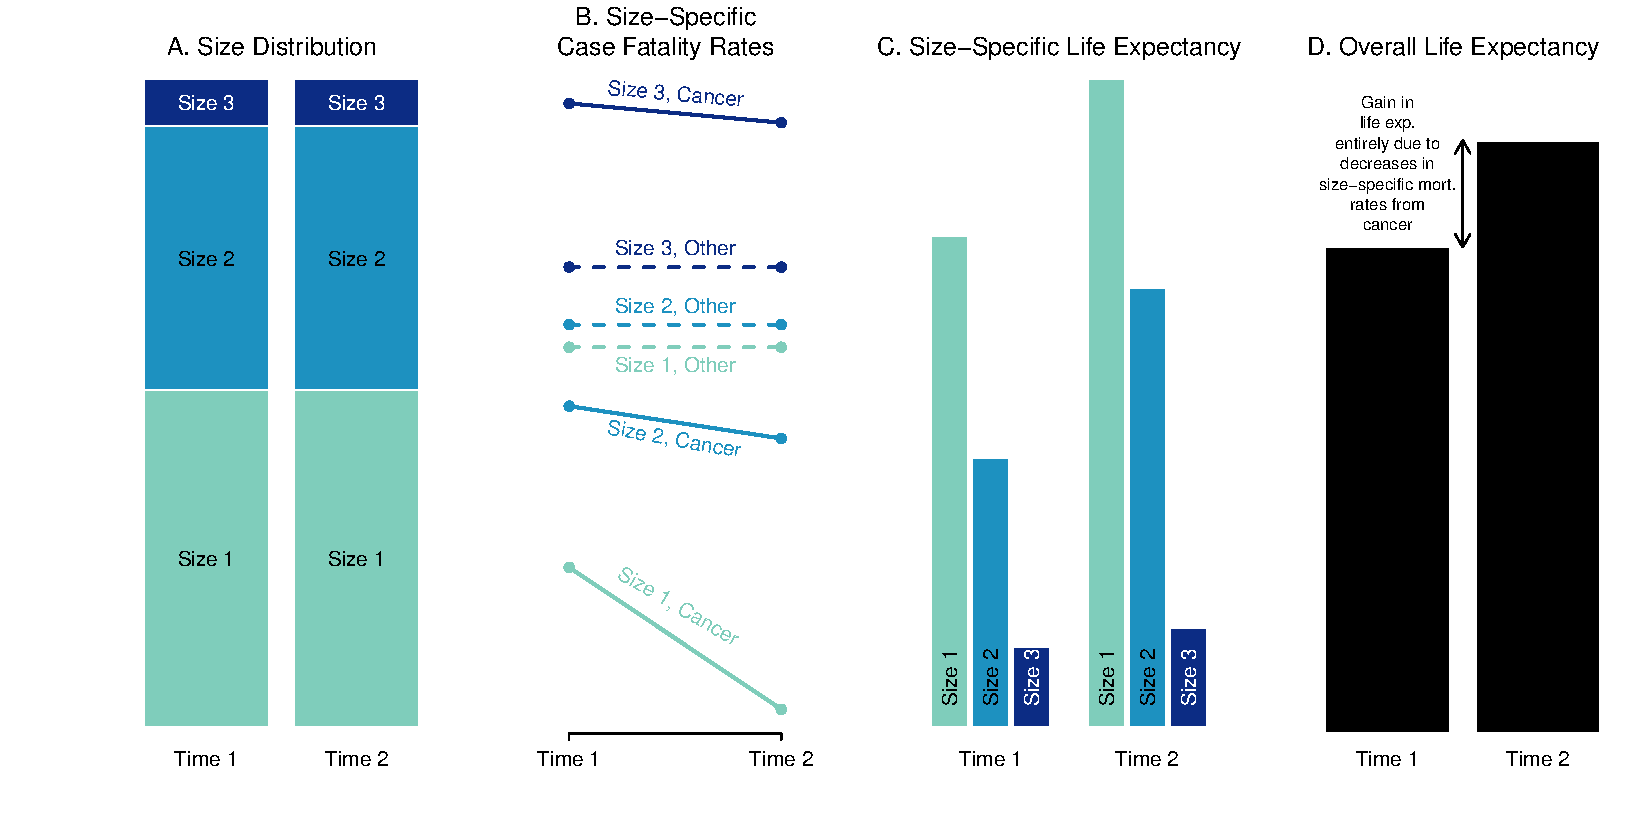
\includegraphics[width=\linewidth]{figure1.pdf}
\caption{Changes in the gain in life expectancy depend on three factors.  (A) Changes in the tumor size distribution at cancer diagnosis, (B) tumor size-specific case fatality rates from breast cancer, and (C) tumor size-specific life expectancy.} 
\label{fig:simple_case}
\end{center}
\end{figure}

\section{Decomposition by Tumor Size and Case Fatality Rates from
  Breast Cancer and Other Causes of Death}
Let $\pi_i(t)$ and $e_i(a,t)$ be the proportion of patients and the
life expectancy for cancer patients with tumor size $i$ (i.e., $<1$
cm, 1-2 cm, 2-3 cm, 3-5 cm, and 5+ cm.) at age $a$ and time $t$,
respectively. That is, $e_i(a,t)$ represents tumor-size-specific life
expectancy. The overall life expectancy at age $a$ time $t$ is given
by
\begin{eqnarray}
  e(a,t)=\sum_{i=1}^{5}\,\pi_i(t)\,e_i(a,t) \notag
\end{eqnarray}
where $\sum_{i=1}^{5}\,\pi_i=1$. 

The change in life expectancy at age $a$ between times $t_1$ and $t_2$
by tumor sizes can be decomposed using the methodology of \cite{Kitagawa55}:
\begin{align}
  e(a,t_2)-e(a,t_1)&=\sum_{i=1}^{5}\left[\,\pi_i(t_2)\,e_i(a,t_2)- \pi_i(t_1)\,e_i(a,t_1)\right]  \notag\\
  \hspace{-0.7in} &=\sum_{i=1}^{5}\left[\pi_i(t_2)-\pi_i(t_1)
  \right]\left[\frac{e_i(a,t_1)+e_i(a,t_2)}{2}\right]+ \notag\\
  &\phantom{=}\sum_{i=1}^{5}\left[e_i(a,t_2)-e_i(a,t_1)
  \right]\left[\frac{\pi_i(t_1)+\pi_i(t_2)}{2}\right].
 \label{eqn:decomp.basic}
\end{align}
 
Equation~\ref{eqn:decomp.basic} quantifies how much of the change in life
expectancy at age $a$ between times $t_1$ and $t_2$ is due to: [a]
shifts in the share of cancer tumor size (first term) and [b] changes
in tumor-size-specific life expectancy (second term).

We can further decompose the second term in the above equation by
cause of death. In doing so, we can quantify how much of this change
in tumor-size-specific cancer life expectancy,
$e_i(a,t_2)-e_i(a,t_1)$, is due to improvements in cancer mortality
and competing causes of death.  Using the approach developed in
\cite{BelPreCan08},
\begin{eqnarray}
e_i(a,t_2)-e_i(a,t_1)=\sum_{j=1}^{k} \sum_{s=x}^{\omega}\left[L_{s,i,j}(t_2)-L_{s,i,j}(t_1) \right] \left[\frac{L_{s,i,-j}(t_2)+L_{s,i,-j}(t_1) }{2n} \right]
\label{eqn:causedecomp}
\end{eqnarray}
where $i$ corresponds to tumor size, $j$ is cause-specific mortality
among patients diagnosed with tumor size $i$ (e.g., $j=1$ is cancer, 
$j=2$ is cardiovascular, etc.; negative indexes correspond to all but the cause, when $j=1$ then  $-j$ is all but cancer, when $j=2$ then  $-j$ is all but cardiovascular, etc), $s$ is age, $\omega$ is the starting
age of the oldest age interval, $n$ is the width of the age interval,
and $L_s$ are person-years lived in the life table.

We perform the decomposition starting at age 40, so the final
decomposition equation is given by:
\begin{align*}
  e(40,t_2)-e(40,t_1)&=\sum_{i=1}^{5}\left[\,\pi_i(t_2)\,e_i(40,t_2)- \pi_i(t_1)\,e_i(40,t_1)\right] \notag \\
                     &=\sum_{i=1}^{5}\left[\pi_i(t_2)-\pi_i(t_1) \right]\left[\frac{e_i(40,t_1)+e_i(40,t_2)}{2}\right]+\sum_{i=1}^{5}\left[\mathtt{Diff_e} \right]\left[\frac{\pi_i(t_1)+\pi_i(t_2)}{2}\right],
\end{align*}
where $\mathtt{Diff_e}$ is given by \eqref{eqn:causedecomp} evaluated at $a=40$.\\


\section{Decomposition by Tumor Size, Case Fatality Rates from
  Breast Cancer and Other Causes of Death, and Age Group}
Let $\pi_{i,a}(t)$ be the proportion of cancer patients with tumor
size $i$ (i.e., $<1$ cm, 1-2 cm, 2-3 cm, 3-5 cm, and 5+ cm.). These
proportions can be computed by age group such that
$\pi_i(t)=\sum_{a\in\mathcal{A}}\pi_{i,a}(t)$ and
$\sum_{i=1}^{5}\,\pi_i=1$, where $\mathcal{A}$ is the set of age
groups (e.g., $a=1$ represents 40-49 years old, $a=2$ represents 50-59
years old, $\dots$, $a=7$ represents 100+ years old).  Then, the
change in life expectancy at age $a$ between times $t_1$ and $t_2$ can
be estimated as:
\begin{align*}
  e(40,t_2)-e(40,t_1)&=\sum_{i=1}^{5}\left[\,\pi_i(t_2)\,e_i(40,t_2)- \pi_i(t_1)\,e_i(40,t_1)\right] \\
                     &=\sum_{i=1}^{5} \left[\sum_{a=1}^{7}\pi_{i,a}(t_2)\,e_i(40,t_2)- \sum_{a=1}^{7}\pi_{i,a}(t_1)\,e_i(40,t_1) \right]\\
                     &=\sum_{i=1}^{5}\left[\pi_{i,1}(t_2)\,e_i(40,t_2)-
                       \pi_{i,1}(t_1)\,e_i(40,t_1)\right] +\\
                     &\hspace{0.18in}\sum_{i=1}^{5}\left[\pi_{i,2}(t_2)\,e_i(40,t_2)- \pi_{i,2}(t_1)\,e_i(40,t_1)\right] + \\
  &\phantom{=\Sigma}\vdots \\
                     &\hspace{0.18in}\sum_{i=1}^{5}\left[\pi_{i,7}(t_2)\,e_i(40,t_7)- \pi_{i,7}(t_1)\,e_i(40,t_1)\right]. \notag 
 \end{align*}


Each summation in the above equation can be written as (see equation
 \eqref{eqn:decomp.basic}):
\begin{multline}
  e(40,t_2)-e(40,t_1)= \\
  \sum_{i=1}^{5}\left[\pi_{i,1}(t_2)-\pi_{i,1}(t_1) \right]\left[\frac{e_i(40,t_1)+e_i(40,t_2)}{2}\right]+\sum_{i=1}^{5}\left[e_i(40,t_2)-e_i(40,t_1) \right]\left[\frac{\pi_{i,1}(t_1)+\pi_{i,1}(t_2)}{2}\right] +\\
  \sum_{i=1}^{5}\left[\pi_{i,2}(t_2)-\pi_{i,2}(t_1) \right]\left[\frac{e_i(40,t_1)+e_i(40,t_2)}{2}\right]+\sum_{i=1}^{5}\left[e_i(40,t_2)-e_i(40,t_1) \right]\left[\frac{\pi_{i,2}(t_1)+\pi_{i,2}(t_2)}{2}\right] +\\
  \vdots \\
  \sum_{i=1}^{5}\left[\pi_{i,7}(t_2)-\pi_{i,7}(t_1) \right]\left[\frac{e_i(40,t_1)+e_i(40,t_2)}{2}\right]+\sum_{i=1}^{5}\left[e_i(40,t_2)-e_i(40,t_1) \right]\left[\frac{\pi_{i,7}(t_1)+\pi_{i,7}(t_2)}{2}\right] =\\
  \sum_{i=1}^{5}\left[\mathtt{Diff_{\pi,1}} \right]\mathtt{\bar{e}_i} + \sum_{i=1}^{5}\left[\mathtt{Diff_{\pi,2}} \right]\mathtt{\bar{e}_i} + 
  \dots +
 \sum_{i=1}^{5}\left[\mathtt{Diff_{\pi,7}} \right]\mathtt{\bar{e}_i} +\sum_{i=1}^{5}\left[e_i(40,t_2)-e_i(40,t_1)\right]\left[\frac{\pi_i(t_1)+\pi_i(t_2)}{2}\right]
\label{agedec}
\end{multline}
where $\mathtt{Diff_{\pi,a}}=\pi_{i,a}(t_2)-\pi_{i,a}(t_1)$ for $a=1,\dots,7$ and $\mathtt{\bar{e}_i}=\frac{e_i(40,t_1)+e_i(40,t_2)}{2}$.

The first seven terms of equation \eqref{agedec}, those involving $\mathtt{Diff_{\pi,1}}$ through $\mathtt{Diff_{\pi,7}}$,  correspond to the
contribution of changes in the share of tumor size by age group to
changes in cancer life expectancy between times $t_1$ and $t_2$. We
can additionally estimate the contribution of cancer-specific
mortality rates to changes in tumor-size-specific life expectancy by
age. The last term of \eqref{agedec} can be written as (see equation
\eqref{eqn:causedecomp}):
\begin{align}
  e_i(40,t_2)-e_i(40,t_1)&=\sum_{j=1}^{k} \sum_{s=40}^{49}\left[L_{s,i,j}(t_2)-L_{s,i,j}(t_1) \right] \left[\frac{L_{s,i,-j}(t_2)+L_{s,i,-j}(t_1) }{2n} \right] + \notag\\
  &\phantom{=}\sum_{j=1}^{k} \sum_{s=50}^{59}\left[L_{s,i,j}(t_2)-L_{s,i,j}(t_1) \right] \left[\frac{L_{s,i,-j}(t_2)+L_{s,i,-j}(t_1) }{2n} \right] + \notag\\
  &\phantom{=  .}\vdots \notag\\
  &\phantom{=}\sum_{j=1}^{k} \sum_{s=100}^{\omega}\left[L_{s,i,j}(t_2)-L_{s,i,j}(t_1) \right] \left[\frac{L_{s,i,-j}(t_2)+L_{s,i,-j}(t_1) }{2n} \right] .
\end{align}

\section{Assuming Constant Mortality Within Age Intervals}
Let $M_{a,a+n}$ represent the mortality rate between ages $a$ and
$a+n$. Then
\begin{equation}
l_{a+n}=e^{-\int_a^{a+n}\mu(s)\,ds}=e^{-n\,M_{a,a+n}}.\notag
\end{equation}
We can then estimate the person-years lived between ages $a$ and $a+n$
as
\begin{equation}
_nL_{a}=l_a\,\int_a^{a+n} e^{-M_{a,a+n}(s-a)} ds=l_a \left(\frac{-1}{M_{a,a+n}}(e^{-n\,M_{a,a+n}}-1) \right).
\label{Lx}
\end{equation}
If, for example, age intervals are 5 years wide, equation \eqref{Lx}
equals
\begin{equation}
_5L_{a}=l_a \left(\frac{-1}{M_{a,a+5}}(e^{-5\,M_{a,a+5}}-1) \right).\notag
\end{equation}
For the last age group (e.g., $\geq$100 years), we can assume there
are no person-years lived beyond a certain time (say no more than 10
years) to compute $_+L_{100}$ as
\begin{equation}
_+L_{100}=l_{100} \left(\frac{-1}{M_{100+}}(e^{-10\,M_{100+}}-1) \right).\notag
\end{equation}

%Consider tumor size $i$.  The change
%in life expectancy at age $x$ between times $t_1$ and $t_2$ can be
%decomposed as (Kitigawa 1955): 
%\begin{equation}
% e_i(x,t_2)-e_i(x,t_1) = \sum_{j=1}^k \int_x^\infty \left[ p_{i,j}(s,t_2)- p_{i,j}(s,t_1)\right] \left[ \frac{p_{i,-j}(s,t_1)+p_{i,-j}(s,t_2)}{2} \right]\,ds, \notag
%\end{equation}
%where $p_{i,j}(s,t)$ is the probability of surviving from birth to age
%$s$ for cancer patients with tumor size $i$ cause $j$ at time $t$, and
%$p_{i,-j}(s,t)$ is the analogue survival probability for competing
%causes of death (other than $j$). 

\newpage
\section{Varying Time Intervals Between Diagnosis and Death}
\spacingset{1}
\begin{center}
  \begin{table}[h]
\begin{tabular}{@{}l rrrrr@{}}
  \toprule
Time & & Gain in & Earlier & \multicolumn{2}{c}{Advancements in Treatment of}\\
 \cmidrule(l{1em}r{1em}){5-6}
Interval &  & Life Expectancy & Detection  & Breast Cancer   & Other Diseases  \\ 
(Yrs) &  Period & (Yrs) & (Yrs) & (Yrs) & (Yrs) \\
  \midrule
  8 & 1975-2002 & 11.23 & 3.15 (28\%) & 7.07 (63\%) & 1.03 (9\%) \\ 
    9 & 1975-2002 & 10.93 & 3.09 (28\%) & 6.76 (62\%) & 1.09 (10\%) \\ 
   10 & 1975-2002 & 10.69 & 2.99 (28\%) & 6.57 (61\%) & 1.15 (11\%) \\ 
   11 & 1975-2002 & 10.38 & 2.78 (27\%) & 6.27 (60\%) & 1.35 (13\%) \\ 
   12 & 1975-2002 & 10.28 & 2.65 (26\%) & 6.05 (59\%) & 1.59 (15\%) \\ 
   \bottomrule
\end{tabular}
\caption{Gain in Life Expectancy and Contribution from Earlier
  Detection, Advancements in Breast Cancer Treatment, and Advancements
  in Treatment of Other Diseases, Varying Incidence-Based Case
  Fatality Rate Window Length.  Note: Yrs=years.}
\end{table}
\end{center}

\begin{center}
  \begin{table}[h]
\begin{tabular}{@{}l rrrrr@{}}
 Time & & Gain in & Earlier & \multicolumn{2}{c}{Advancements in Treatment of}\\
 \cmidrule(l{1em}r{1em}){5-6}
Interval &  Period& Life Expectancy & Detection  & Breast Cancer   & Other Diseases  \\ 
  \midrule
  8 & 1975-2002 & 11.23 & 3.15 (28\%) & 7.07 (63\%) & 1.03 (9\%) \\ 
    9 & 1975-2002 & 10.93 & 3.09 (28\%) & 6.76 (62\%) & 1.09 (10\%) \\ 
   10 & 1975-2002 & 10.69 & 2.99 (28\%) & 6.57 (61\%) & 1.15 (11\%) \\ 
   11 & 1975-2002 & 10.38 & 2.78 (27\%) & 6.27 (60\%) & 1.35 (13\%) \\ 
   12 & 1975-2002 & 10.28 & 2.65 (26\%) & 6.05 (59\%) & 1.59 (15\%) \\ 
   \bottomrule
\end{tabular}
\caption{Gain in Life Expectancy and Contribution from Earlier
  Detection, Advancements in Breast Cancer Treatment, and Advancements
  in Treatment of Other Diseases, Varying Incidence-Based Case
  Fatality Rate Window Length.  Note: Yrs=years.}
\end{table}
\end{center}

\newpage
\spacingset{1} \pdfbookmark[1]{References}{References}
\bibliography{cancer}
\end{document}



